\chapter{Validation} \label{validation}

\bigskip \bigskip

Validation of a knowledge graph refers to the process of verifying the accuracy, completeness, and consistency of the data contained within the graph. A knowledge graph is a complex network of interrelated data points, and it is important to ensure that the data is reliable and consistent to ensure that the knowledge graph can be used effectively. Validation of a knowledge graph is particularly important in applications such as risk assessment, where inaccurate data can have significant consequences in terms of safety. For example, if the knowledge graph used to access a particular machine lacks a certain hazard in its hazard pool, or if the checklist of a certain hazard misses certain point, then the risk stays unmitigated which could be catastrophic. Validation can also be an ongoing process from the perspective of a risk assessment. As machines are evolving, standards are updating, the knowledge graph needs to be updated to incorporate all the new hazards and preventive measures that comes up with time. Thus, ongoing validation is also important to ensure that the knowledge graph remains accurate and up-to-date as new data becomes available.

\paragraph{} For this thesis, validation is mainly restricted to face validity of the knowledge graph and validation against an expert. This is inspired from the two step validation as mentioned in \cite{sim} which suggests that a model should have high face validity and good quality of output. These are divided into two separate sections (\ref{face_validity} and \ref{expert_validity}). Apart from this, the completeness of the knowledge model can be checked by re-creating a complete TRF (checklist) of the standard by querying the model and getting this TRF checked by an expert. But due to shortage in time it was not possible to get the complete TRF checked. However, the hasClause relation is used in the face validity section which can be checked with the standard to see that all the clauses have been included in the knowledge model with some depth for the respective clauses. Thus, completeness is mostly self-validated. 

\section{Face validity} \label{face_validity}
Face validity is the type of validity that refers to whether the results from the model built appears reasonable when the model is used and that the model does what it is supposed to do. Face validity makes sure that there are no clear mistakes in the model structure, whether the concepts and relations are correctly converted to SPO triples and that the model gives predictable output when queried. While these tests are mostly subjective or implemented through apparently self-validating experiments, they serve as a first sanity check for model correctness.

\paragraph{} Alongside of checking for face validity, the model is also updated to fix errors. So the approach taken was to go through the model thoroughly with the safety standard ISO 12100. This would help to examine how coherent the model is with the safety standard and that it covers the important aspects of the safety standard. It would also help to fix any missing relationships or connections or any contradictory triplets in the model. An important point should be noted here that the model is not checked for completeness but it is checked for correctness of the concepts and relations modelled.

\paragraph{} The test starts with a query for the relation hasClause. This would easily give all the important concepts present in the model that are taken from the standard and have a clause number corresponding to the standard. 

% \bigskip\bigskip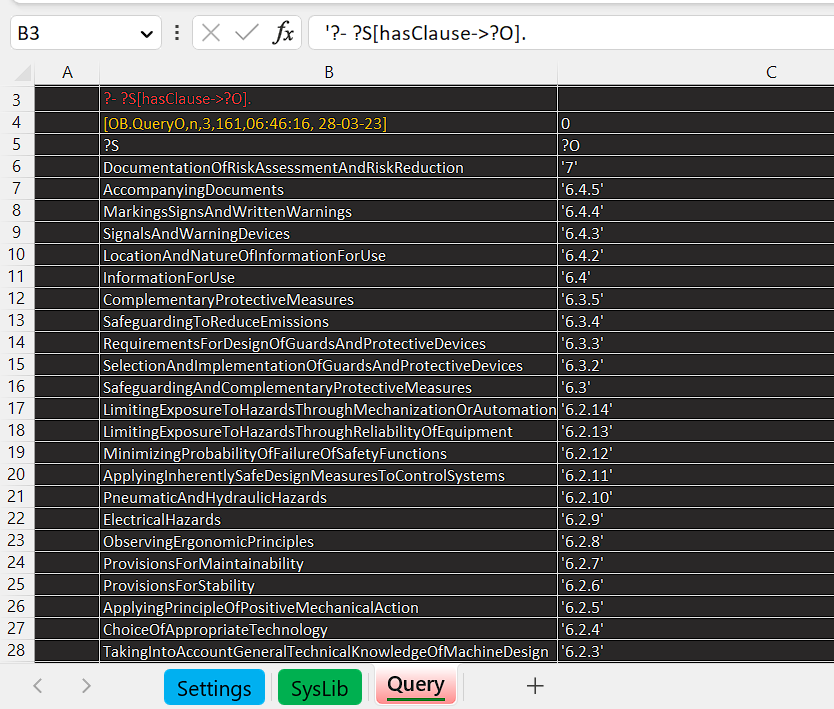
\includegraphics[width=\textwidth]{img/hasClause.png}

\bigskip\bigskip \adjustimage{width=\textwidth, center, caption={Query on the relation hasClause}, label={fig21}, nofloat=figure, vspace=\bigskipamount}{img/hasClause.png}

\paragraph{} Then each concept from clause 4 to clause 7 are queried for. Each query are continued till the depth it can go. And along with this the safety standard ISO 12100 is also referred for each clause to validate the correctness of the data. 

\paragraph{} For a few concepts, it is found that different terms are used for the same concept which does not give good results on query. Synonyms are used throughout the standard and since the knowledge graph is developed using a semi-automated approach, these synonyms are copied in the model as well. For example, the term machine and machinery means the same concept machine. But they were two different concepts in the knowledge graph. This gives dual result when there is a query related to machine. So, these synonyms are replaced with an uniform concept name throughout the model, for example "Machine" in this case. A few other similar occurrences of synonyms of other concepts are found as well and are replaced accordingly.

\section{Validation against an expert} \label{expert_validity}
Expert validation of a knowledge graph for industrial risk assessment is an important step in ensuring its accuracy and reliability. But it may not always be an easy task to achieve. There are several reasons that could make the task of validating the knowledge graph against an expert a challenging one.

\paragraph{} The knowledge graph is complex, with many concepts and relationships between them. Experts may need to spend significant time and effort understanding the knowledge graph if they were to go through each relations. Also, a semantic model is highly subjective with a lot of modelling possibilities. So it is nearly impossible for the domain expert to go through each relation and come up with a quantitative review. For this reason, face validity was performed. 

\paragraph{} Depending on the tools and technologies used to build the knowledge graph, experts may need to have some technical expertise to evaluate it effectively. And it is not always the case that an expert of machinery safety can understand how OntoBroker works or what is a knowledge model in general and how the input data is processed. This can be a barrier or maybe overwhelming for an expert to evaluate the knowledge graph in the first place.

\paragraph{} Also experts may have limited time available to review the knowledge graph, especially if they have other responsibilities or projects to manage. This can make it difficult to provide detailed feedback and suggestions for improvement. For this reason, the validation should be planned well so that it is easy for the expert to give a quantifiable review of the model as well as it is the fastest way of validation possible.

\paragraph{} The relation haveChecklistQuestions would provide the questions that can be used in a checklist for risk assessment. A few sections are selected and for each of them the checklist questions are queried from the model. These questions are then transferred to a TRF (Test Report Form). An example of the checklist questions for Noise Hazard is shown below. 

% \bigskip\bigskip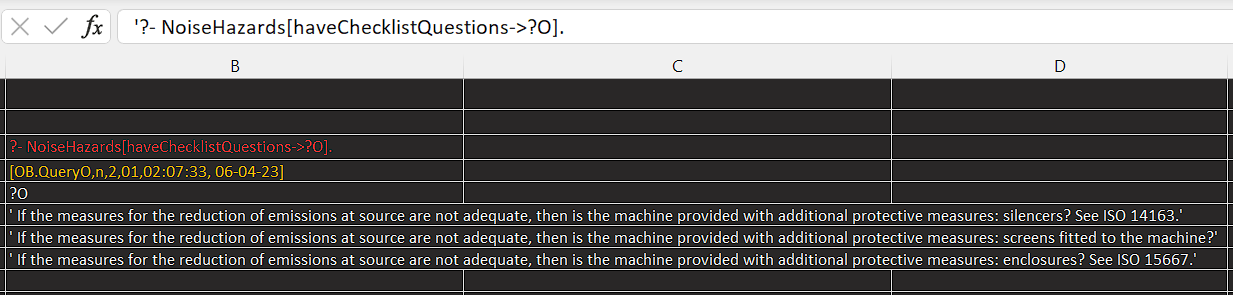
\includegraphics[width=\textwidth]{img/NoiseHazards_Checklist.png}

 \bigskip\bigskip \adjustimage{width=\textwidth, center, caption={Query for the checklist questions for noise hazard}, label={fig22}, nofloat=figure, vspace=\bigskipamount}{img/NoiseHazards_Checklist.png}

\paragraph{} The questions are separated per section and the corresponding clause number are also mentioned which would make them easier to refer from the ISO 12100. The clause number can easily be queried with the relation hasClause. The TRF is a document that is used everyday by an expert to perform risk assessment, so the format of the document is well known to him/her. Also it is very easy to transfer the checklist questions queried from the knowledge graph to a TRF. It would involve just copy and paste of the data. So now the expert can easily look at questions for the corresponding sections of the TRF and comment on its correctness. This is the easiest and the fastest way in which the output from the model could be validated by an expert. It would also save time and effort of an expert. An example page of the TRF output from the knowledge graph is shown below in Figure \ref{fig23}.

% \bigskip\bigskip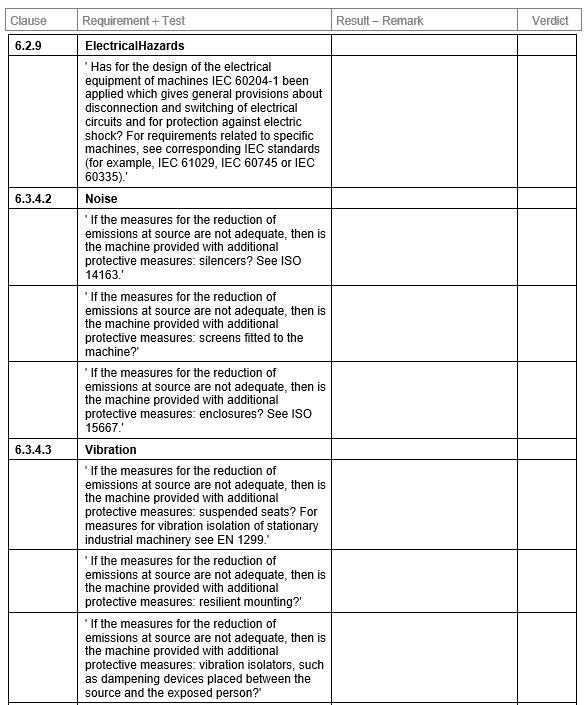
\includegraphics[width=\textwidth]{img/TRFoutput_from_KG.png}

\bigskip \adjustimage{width=\textwidth, center, caption={Checklist questions in TRF format}, label={fig23}, nofloat=figure, vspace=\bigskipamount}{img/TRFoutput_from_KG_2.png}

\paragraph{} The evaluation sheet is divided into two sections, namely, correctness of the checklist from the knowledge model and usefulness of the knowledge model. Validation would be incomplete without quantifiable results as they provide a clear and objective way to measure the performance or accuracy of the model. The expert is provided with an evaluation sheet along with the TRF output. The expert can then check for correctness of the TRF output for the selected clauses. The expert can rate between a score of 1 to 4 for each of the selected clause. The filled evaluation sheet is attached below in Figure \ref{fig24}.

\bigskip \adjustimage{width=\textwidth, center, caption={Evaluation sheet for the correctness of the knowledge model}, label={fig24}, nofloat=figure, vspace=\bigskipamount}{img/checklist_evaluation.png}

\paragraph{} The clauses where the knowledge model is said to not fully reach expectations are due to referencing of another standard. The external standard is referenced only for the first point but they need to be referenced for all points. The input data for these checklist questions comes from a previous risk assessment where the references were not such. But with this review from the expert, the knowledge model is also updated to include the reference. 

\paragraph{} After validating the correctness, it is also important to review the structure of the model for its usefulness in risk assessment. The usefulness of the knowledge model is evaluated after a brief explanation of the implementation of the knowledge graph to two experts. The points for usefulness of the model is based on the implementation of the model in current risk assessment which is described in chapter \ref{implementation} of this thesis. The implementation of the knowledge graph is demonstrated to the experts and they could rate between a score of 1 to 4 for each use case. Similar to the rating used to evaluate the correctness of the checklist generated from the model. The final scores are averaged in the filled evaluation sheet which is attached below in Figure \ref{fig25}.

% \bigskip\bigskip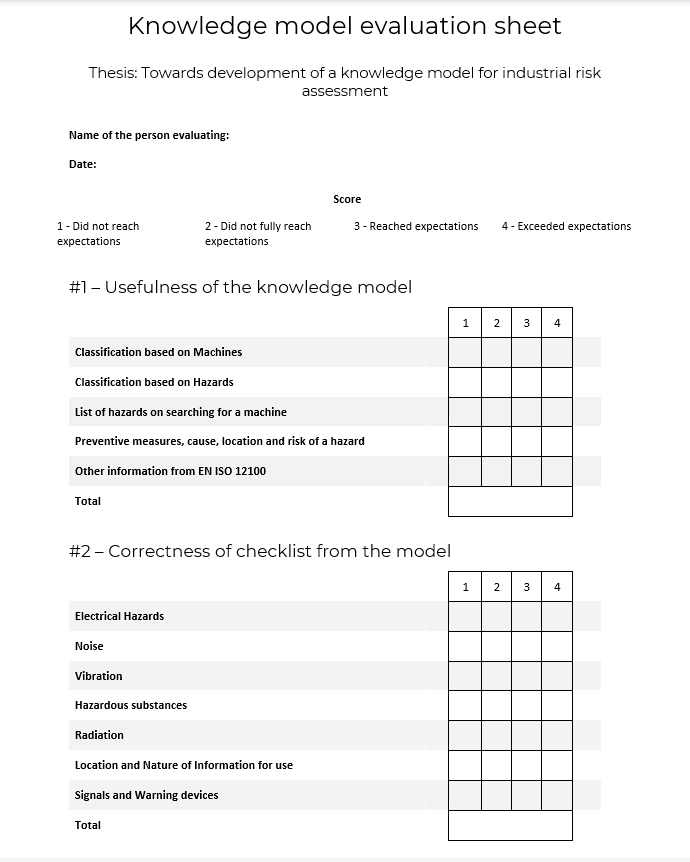
\includegraphics[width=\textwidth]{img/evaluation_sheet.png}

\bigskip\bigskip \adjustimage{width=\textwidth, center, caption={Evaluation sheet for the usefulness of the knowledge model}, label={fig25}, nofloat=figure, vspace=\bigskipamount}{img/checklist_review.png}